\documentclass[conference]{IEEEtran}
\IEEEoverridecommandlockouts

\usepackage{cite}
\usepackage{amsmath,amssymb,amsfonts}
\usepackage{algorithmic}
\usepackage{graphicx}
\usepackage{textcomp}
\usepackage{xcolor}
\usepackage{hyperref}
\usepackage{placeins}

\def\BibTeX{{\rm B\kern-.05em{\sc i\kern-.025em b}\kern-.08em T\kern-.1667em\lower.7ex\hbox{E}\kern-.125emX}}

\begin{document}
    % Title
    \title{Human Activity Recognition Using Smartphones\\}

    % Authors
    \author{\textit{Kalos Lazo (100\%), Lucas Carranza (100\%), Benjamín Soto (100\%), José Osnayo}}
\maketitle

\section{Introducción}
En el presente documento se discute acerca de la resolución de un problema de clasificación supervisada a partir de un estudio realizado a un grupo de voluntarios de entre $19$ y $48$, mientras realizaban actividades cotidianas: \textit{caminar, subir escaleras, bajar escaleras, sentarse, levantarse y acostarse} se obtuvieron datos del acelómetro y giroscopio embebido sus teléfonos inteligentes: \textit{Samsung Galaxy SII}. Los datos fueron convertidos usando la librería TsFresh para extraer las características de las series temporales más importantes. Finalmente se usaron dos modelos de clasificación para predecir la actividad realizada según las características de la serie temporal.

\section{Conjunto de Datos}
\subsection{Exploración del Dataset}
Los datos utilizados en este proyecto contienen información extraída del teléfono: \textit{acelerómetro y giroscopio}. Esta información se provee en un archivo de extensión \texttt{.h5} que indica que es un formato jerárquico \texttt{HDF} y sirve para múltiples datasets. Para la data de entrenamiento se incluyeron consigo, en su jerarquía, 10 datasets con 7352 entradas que indican lo siguiente:

\begin{table}[htbp]
    \caption{Descripción de Variables}
    \begin{center}
        \begin{tabular}{|l|l|}
        \hline
        \textbf{Variable} & \textbf{Descripción} \\
        \hline
        \texttt{body\_acc\_x} & Señal de aceleración del cuerpo en el eje X.\\
        \hline
        \texttt{body\_acc\_y} & Señal de aceleración del cuerpo en el eje Y.\\
        \hline
        \texttt{body\_acc\_z} & Señal de aceleración del cuerpo en el eje Z.\\
        \hline
        \texttt{body\_gyro\_x} & Velocidad angular medida en el eje X.\\
        \hline
        \texttt{body\_gyro\_y} & Velocidad angular medida en el eje Y. \\
        \hline
        \texttt{body\_gyro\_z} & Velocidad angular medida en el eje Z. \\
        \hline
        \texttt{total\_acc\_x} & Señal de aceleración total en el eje X. \\
        \hline
        \texttt{total\_acc\_y} & Señal de aceleración total en el eje Y. \\
        \hline
        \texttt{total\_acc\_z} & Señal de aceleración total en el eje Z. \\
        \hline
        \texttt{y} & Etiquetas de actividad del 1 al 6. \\
        \hline
        \end{tabular}
        \label{tab1}
    \end{center}
\end{table}

Cada dataset (excepto \texttt{y}) cuenta con 128 columnas, donde cada una corresponde a la medida de cada variable en cierta unidad de tiempo.
Para la data de testing se incluyeron las mismas variables a excepción de \texttt{y} con 2947 entradas.

\subsection{Análisis de Frecuencias}
Analizamos las frecuencias de cada clase utilizando la librería \textit{Seaborn} para graficar el histograma.
\begin{figure}
    \centering
    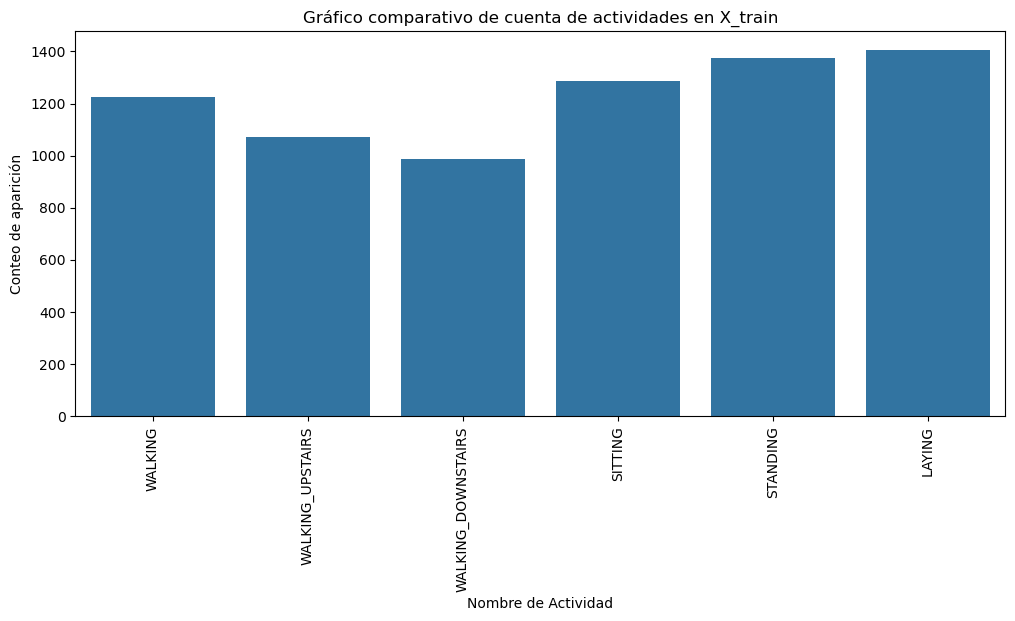
\includegraphics[width=\linewidth]{class_freq.png}
    \caption{Histograma de Frecuencias de Clases}
    \label{fig1}
\end{figure}
Observamos que las frecuencias son casi equivalentes, por lo que no hay que tener consideraciones especiales por desbalanceo.

\subsection{Extracción de Features}
Para poder utilizar los datos para realizar la clasificación necesitamos convertir las series temporales a un conjunto de características. Para realizar esto se usó la librería TsFresh con su función \texttt{extract\_features} con los parámetros mínimos. Esto convirtió cada dataset de 128 timestamps a 9 características, por lo que se concatenaron para obtener un dataset de entrenamiento y testing de 81 características.

\begin{table}[htbp]
    \caption{Descripción de Características}
    \begin{center}
        \begin{tabular}{|l|l|}
        \hline
        \textbf{Característica} & \textbf{Descripción} \\
        \hline
        \texttt{sum\_values} & Suma de valores de la serie temporal.\\
        \hline
        \texttt{median} & Mediana de los valores.\\
        \hline
        \texttt{mean} & Media aritmética de los valores.\\
        \hline
        \texttt{standard\_deviation} & Desviación estándar de los valores.\\
        \hline
        \texttt{variance} & Varianza de los valores. \\
        \hline
        \texttt{root\_mean\_square} & Raíz de la media de los cuadrados. \\
        \hline
        \texttt{maximum} & Valor máximo de la serie temporal. \\
        \hline
        \texttt{absolute\_maximum} & Valor máximo absoluto de la serie. \\
        \hline
        \texttt{minimum} & Valor mínimo de la serie temporal. \\
        \hline
        \end{tabular}
        \label{tab2}
    \end{center}
\end{table}

\section{Metodología}
% Explanation of the model, loss functions, and regularization techniques
Se utilizaron principalmente dos modelos en este proyecto: KNN usando K-DTree y Regresión Logística con función Softmax.

\subsection{Justificación}
La razón por la que se usó KNN fue por la facilidad de su implementación para clasificación de múltiples clases, y se utilizó un KD-Tree para garantizar su eficiencia, ya por el contrario se deben calcular las distancias entre más 7000 puntos de 81 dimensiones. Finalmente, debido a que el número de dimensiones no es demasiado grande, no sufrimos del caso de \textit{Curse of Dimensionality}, por lo que es un modelo viable para este caso.

Asimismo, se probó la clasificación utilizando Decision Tree. Sin embargo debido a que los datos eran continuos en vez de discretos, el punto de splitting óptimo fue difícil de calcular. Esto resultó en una predicción sub-óptima con precisión de testing inferior a 20\% con alta varianza, a pesar de una precisión óptima de validación. Esto acompañado con el hecho de que se solían predecir solo 3 de las 6 clases, sugiere que este modelo generaba \textit{overfitting} con sesgo hacia las ciertas clases. Esto nos llevó a descartar este modelo para este trabajo, y proseguir con otros.

Por ende, para aprovechar los datos continuos se utilizó Regresión Logística. Sin embargo, debido a que el modelo visto en clase solo permite clasificación binaria, se implementó una función Softmax para reemplazar la función Sigmoide, lo cual permite realizar clasificación Multinomial. A diferencia del KNN, este modelo sí requiere de entrenamiento, por lo que para garantizar su eficiencia se realizó una experimentación extensiva.

\subsection{KNN}


\subsection{Regresión Logística}
La Regresión Logística usando Softmax requiere utilizar funciones diferentes a las vistas en clase. A continuación se explicarán las fórmulas que difieren de la clasificación binaria:
\begin{itemize}
\item \textbf{One-hot encoding:}
Para poder aplicar las funciones de Loss y las derivadas al igual que en Regresión Logística binaria, necesitamos codificar nuestro vector de clases de tal manera que el valor de $y$ sea 1 si la clase predicha sea correcta, y 0 si es cualquier otra clase diferente. Por este motivo utilizamos \textit{One-hot encoding}, donde hay tantas columnas como clases. Cada fila $y_i$ tiene el valor de 1 en la columna de la predicción correcta, y 0 en todas las demás.

\item \textbf{Función Softmax:}
Esta es la función que reemplaza a la función sigmoide. Matemáticamente, este método sólo extiende la fórmula de regresión logística para $k$ clases. Toma como entrada el vector $z_i$ que corresponde al $x_i$ a predecir, y retorna un vector de las probabilidades de que la entrada pertenezca a cada clase. La suma de las probabilidades de todas las clases siempre suma 1.

\[s(z_i) = \frac{e^{z_i}}{\sum_j^K e^{z_j}}\]

Siendo $K$ el número de clases de nuestro dataset.
La manera en la que funciona es la siguiente:

\[P\{y_i=k\} = \frac{e^{w_kx_i}}{\sum_j^K e^{w_jx_i}}\]

Por lo que obtenemos la probabilidad de que la clase a predecir sea $k$, para cada clase posible. Observamos entonces que $z$ es el producto punto entre los pesos y $x$. Al obtener el valor máximo de las probabilidades, obtenemos la clase de la predicción $\hat{y}$.
\vspace{0.5cm}
\item \textbf{Función Loss:}
A diferencia de la clasificación binaria, donde se usa \textit{Binary Cross Entropy}, en la Regresión Multinomial requerimos de la \textit{Cross Entropy}, que es el equivalente gracias al \textit{One-hot encoding}, solo que funciona para $k$ clases en vez de sólo 2. Solo cuando la precisión sea correcta, $y$ valdrá 1, y valdrá 0 para todas las demás predicciones.
\[\mathcal{L} = -\sum_{i=1}^{n}y_i \cdot log(s_i)\]

Para evitar errores por calcular el logaritmo de $0$, utilizamos un valor epsilon muy pequeño para compensar.

\item \textbf{Derivadas:}
No se modificaron las derivadas de las vistas en clase para Regresión Logística binaria. Como se utiliza \textit{One-hot encoding}, podemos utilizar el principio usado en \textit{Binary Cross Entropy} y aplicarlo para \textit{Cross Entropy} multiclase. Esto nos permite mantener la misma fórmula.
\[\frac{\delta\mathcal{L}}{\delta W} = \frac{1}{n}\sum_{i=1}^n (y_i - \hat{y_i})\cdot (-x_{ij})\]

\item \textbf{Regularización:}
Para prevenir overfitting en el modelo, se agregó regularización L2 (Ridge) a la función Loss y a las derivadas. Para realizar esto se le suma el siguiente término a la función Loss:
\[\frac{\lambda}{2n} ||W||_2^2\]
Y se suma el siguiente término a las derivadas:
\[\frac{\lambda}{n} W\]
Esto penaliza pesos muy grandes y previene el overfitting, haciendo que el valor de la pérdida sea mayor.

\end{itemize}


\section{Implementación}
% Include the link to Colab or GitHub where the implementation can be found, avoiding direct
% code placement in the report. Define a seed to replicate the results. [Optional] Relevant implementation
% details can also be included (error handling, parallelization, etc.).
El código documentado del proyecto se encuentra en el siguiente 
\href{https://github.com/kaloslazo/SupervisedClassification}{Repositorio de Github}


\noindent \textbf{Detalles de implementación:}
\begin{itemize}
\item Durante la experimentación se usó paralelización al momento de realizar la extracción de features. Para la entrega final se eliminó la paralelización para garantizar la integridad y precisión de las características.

\item Se fijó la semilla aleatoria para permitir la replicación de resultados.

\item Se mantuvo en el código la implementación del Decision Tree como evidencia de la experimentación. Sin embargo, como se mencionó en la justificación, su precisión no es representativa de lo logrado en el proyecto por ser sub-óptima. No se usó en el proyecto más que para justificar el uso de los otros modelos por descarte del uso de este mismo.
\end{itemize}


\section{Experimentación}
% Present results with graphs and/or tables, avoiding terminal screenshots
Se experimentaron principalmente con los dos modelos mencionados. Se utilizó K-Fold Cross-Validation con 10 pliegues para calcular la precisión de entrenamiento y validación usando múltiples Bases de Datos. Esto permite un juicio más objetivo sobre la utilidad de los parámetros, y no ocurrirá problema de alta varianza debido al gran número de muestras. Se utilizó la clase \texttt{StandardScaler} de la librería \textit{sklearn} para la normalización de atos. Se justifican los parámetros usados y se exponen los hallazgos a continuación.

\subsection{Experimentación con KNN}
Debido a la naturaleza del algoritmo KNN, el único hiper-parámetro alterable es $k$, o el número de vecinos más cercanos considerados para la predicción. Por este motivo se probaron distintos valores de $k$ para encontrar el punto óptimo, empezando con $k=3$ e incrementando. Evitamos utilizar valores pares, para evitar la posibilidad de empate entre clases y garantizar un resultado único por predicción.

A continuación, las métricas de validación obtenidas con distintos valores de $k$:


\begin{table}[htbp]
    \centering
    \begin{tabular}{cccc}
        \textbf{Fold} & \textbf{Precision} & \textbf{Recall} & \textbf{F1-score} \\
        \hline
        1 & 0.89 & 0.88 & 0.88 \\
        2 & 0.82 & 0.80 & 0.80 \\
        3 & 0.85 & 0.86 & 0.85 \\
        4 & 0.87 & 0.87 & 0.87 \\
        5 & 0.82 & 0.81 & 0.80 \\
        6 & 0.84 & 0.83 & 0.83 \\
        7 & 0.78 & 0.76 & 0.76 \\
        8 & 0.85 & 0.85 & 0.84 \\
        9 & 0.82 & 0.80 & 0.80 \\
        10 & 0.87 & 0.86 & 0.86 \\
        \hline
        \textbf{Promedio} & \textbf{0.841} & \textbf{0.832} & \textbf{0.829} \\
    \end{tabular}
    \caption{Métricas para \( k = 3 \)}
    \label{tab:knn3}
\end{table}

\begin{table}[ht]
    \centering
    \begin{tabular}{cccc}
        \textbf{Fold} & \textbf{Precision} & \textbf{Recall} & \textbf{F1-score} \\
        \hline
        1 & 0.90 & 0.89 & 0.89 \\
        2 & 0.81 & 0.79 & 0.79 \\
        3 & 0.86 & 0.86 & 0.86 \\
        4 & 0.88 & 0.87 & 0.87 \\
        5 & 0.83 & 0.82 & 0.82 \\
        6 & 0.85 & 0.85 & 0.84 \\
        7 & 0.78 & 0.76 & 0.77 \\
        8 & 0.87 & 0.82 & 0.82 \\
        9 & 0.84 & 0.81 & 0.81 \\
        10 & 0.87 & 0.86 & 0.86 \\
        \hline
        \textbf{Promedio} & \textbf{0.849} & \textbf{0.833} & \textbf{0.833} \\
    \end{tabular}
    \caption{Métricas para \( k = 5 \)}
    \label{tab:knn5}
\end{table}

\begin{table}[ht]
    \centering
    \begin{tabular}{cccc}
        \textbf{Fold} & \textbf{Precision} & \textbf{Recall} & \textbf{F1-score} \\
        \hline
        1 & 0.90 & 0.89 & 0.89 \\
        2 & 0.82 & 0.79 & 0.79 \\
        3 & 0.87 & 0.87 & 0.87 \\
        4 & 0.87 & 0.86 & 0.86 \\
        5 & 0.83 & 0.82 & 0.82 \\
        6 & 0.85 & 0.85 & 0.84 \\
        7 & 0.79 & 0.77 & 0.77 \\
        8 & 0.88 & 0.83 & 0.84 \\
        9 & 0.85 & 0.82 & 0.82 \\
        10 & 0.88 & 0.86 & 0.86 \\
        \hline
        \textbf{Promedio} & \textbf{0.854} & \textbf{0.836} & \textbf{0.836} \\
    \end{tabular}
    \caption{Métricas para \( k = 7 \)}
    \label{tab:knn7}
\end{table}

\begin{table}[ht]
    \centering
    \begin{tabular}{cccc}
        \textbf{Fold} & \textbf{Precision} & \textbf{Recall} & \textbf{F1-score} \\
        \hline
        1 & 0.89 & 0.88 & 0.88 \\
        2 & 0.82 & 0.79 & 0.79 \\
        3 & 0.88 & 0.88 & 0.88 \\
        4 & 0.87 & 0.86 & 0.86 \\
        5 & 0.83 & 0.82 & 0.81 \\
        6 & 0.85 & 0.85 & 0.84 \\
        7 & 0.79 & 0.77 & 0.77 \\
        8 & 0.87 & 0.82 & 0.82 \\
        9 & 0.85 & 0.82 & 0.82 \\
        10 & 0.88 & 0.86 & 0.86 \\
        \hline
        \textbf{Promedio} & \textbf{0.853} & \textbf{0.835} & \textbf{0.833} \\
    \end{tabular}
    \caption{Métricas para \( k = 9 \)} 
    \label{tab:knn9}
\end{table}

\begin{figure}[ht]
    \centering
    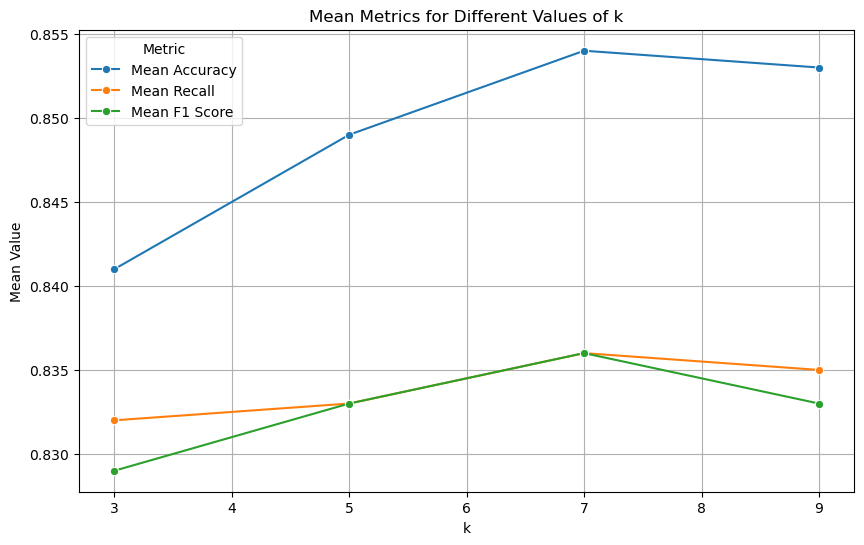
\includegraphics[width=1\linewidth]{kevolve.png}
    \caption{Evolución de las métricas según \(k\)}
    \label{fig:knnmat7}
\end{figure}

\begin{figure}[ht]
    \centering
    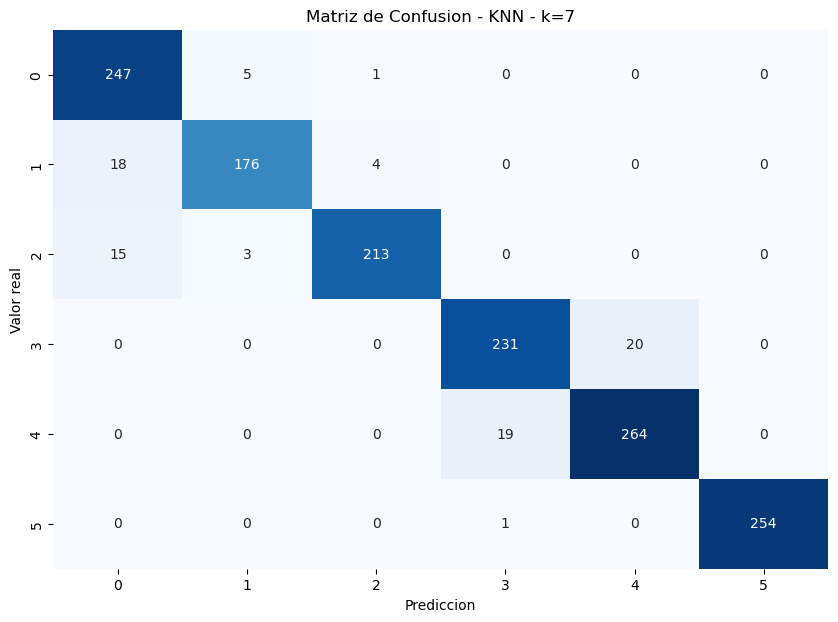
\includegraphics[width=1\linewidth]{knnk7.png}
    \caption{Predicción del mejor parámetro \(k = 7\)}
    \label{fig:knnevolution}
\end{figure}



\FloatBarrier
\subsection{Experimentación con Regresión Logística}
En el caso de la Regresión Logística, contamos con tres parámetros que podemos modificar. El número de epochs, el parámetro de aprendizaje $\alpha$ y el termino de regularización L2 (Ridge) $\lambda$. El número de epochs es un parámetro indirecto (no afecta al modelo directamente), pues con un valor suficientemente alto se llegan a los mismos resultados. Por este motivo lo fijamos en 10mil epochs para la experimentación. Los otros parámetros se encuentran entre 0 y 1, pero se prefieren valores más cercanos a 0. En el caso de $\alpha$, para permitir \textit{fine-tuning} del modelo y evitar saltos grandes, y en el caso de $\lambda$, para evitar \textit{underfitting} por un parámetro de regularización muy grande.

Por este motivo decidimos probar con los siguientes valores de $\lambda$ para comprender el impacto de la regularización sobre la precisión. Se utilizó $\lambda = 0.01$ para probar el caso de una regularización pequeña, y $0.1, 0.2$ para regularizaciones más estrictas. Por cada valor distinto de regularización, probamos con un rango de valores de $\alpha$, que van desde 0.05 (un valor que se mueve lentamente), hasta 0.30 (un valor que da grandes saltos).

A continuación, las métricas de validación obtenidas con distintas combinaciones de $\alpha$ y $\lambda$:

\begin{table}[ht]
    \centering
    \begin{tabular}{ccccc}
        \(\lambda\) & \(\alpha\) & \textbf{Avg. Precision} & \textbf{Avg. Recall} & \textbf{Avg. F1-score} \\
        \hline
        0.01 & 0.05 & 0.891 & 0.882 & 0.887 \\
        0.01 & 0.10 & 0.893 & 0.88 & 0.89 \\
        0.01 & 0.15 & 0.894 & 0.88 & 0.89 \\
        0.01 & 0.20 & 0.895 & 0.88 & 0.89 \\
        0.01 & 0.25 & 0.895 & 0.88 & 0.89 \\
        0.01 & 0.30 & 0.893 & 0.88 & 0.89 \\
        \hline
        0.1 & 0.05 & 0.891 & 0.882 & 0.884 \\
        0.1 & 0.10 & 0.895 & 0.883 & 0.888 \\
        0.1 & 0.15 & 0.894 & 0.883 & 0.887 \\
        0.1 & 0.20 & 0.895 & 0.881 & 0.887 \\
        0.1 & 0.25 & 0.895 & 0.88 & 0.89 \\
        0.1 & 0.30 & 0.894 & 0.88 & 0.89 \\
        \hline 
        0.2 & 0.05 & 0.891 & 0.88 & 0.89 \\
        0.2 & 0.10 & 0.893 & 0.88 & 0.89 \\
        0.2 & 0.15 & 0.893 & 0.88 & 0.89 \\
        0.2 & 0.20 & 0.895 & 0.88 & 0.89 \\
        0.2 & 0.25 & 0.894 & 0.88 & 0.89 \\
        0.2 & 0.30 & 0.889 & 0.88 & 0.89 \\
    \end{tabular}
    \caption{Métricas para Regresión Logística} 
    \label{tab:rl1}
\end{table}

\begin{figure}[ht]
    \centering
    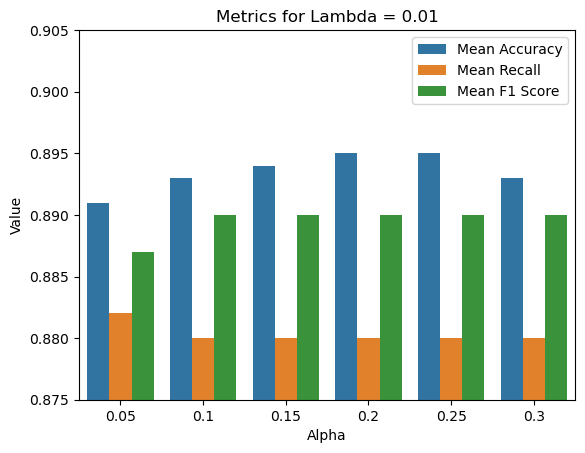
\includegraphics[width=1\linewidth]{01.png}
    \caption{Evolución de las métricas para \(\lambda = 0.01\)}
    \label{fig:rlevolution01}
\end{figure}

\begin{figure}[ht]
    \centering
    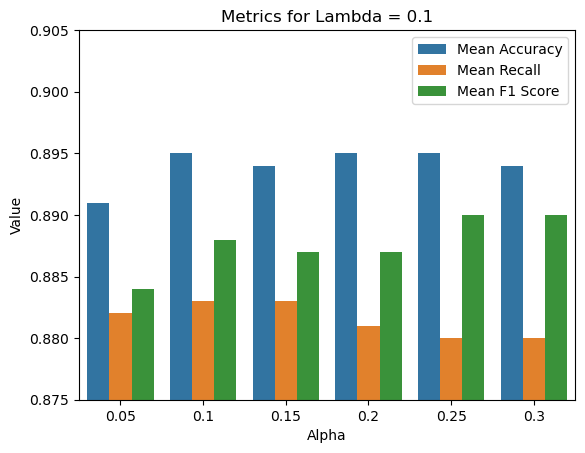
\includegraphics[width=1\linewidth]{1.png}
    \caption{Evolución de las métricas para \(\lambda = 0.1\)}
    \label{fig:rlevolution1}
\end{figure}

\begin{figure}[ht]
    \centering
    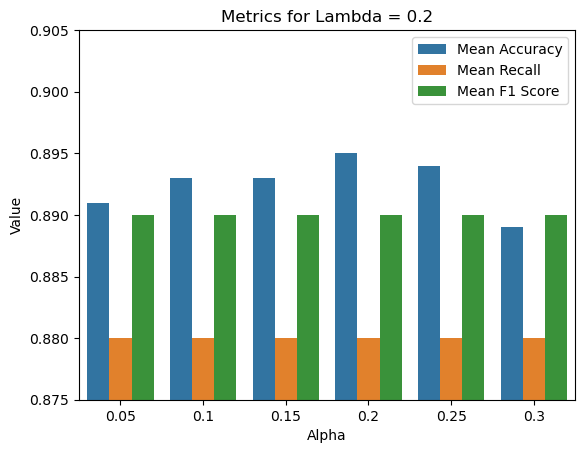
\includegraphics[width=1\linewidth]{2.png}
    \caption{Evolución de las métricas para \(\lambda = 0.2\)}
    \label{fig:rlevolution2}
\end{figure}

\begin{figure}[ht]
    \centering
    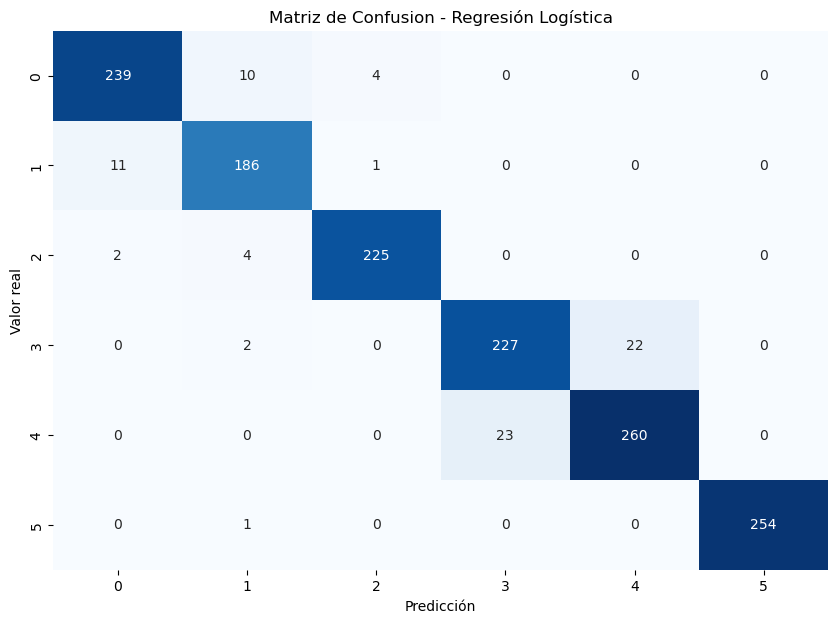
\includegraphics[width=1\linewidth]{log.png}
    \caption{Predicción de unos de los mejores parámetros \(\alpha = \lambda = 0.2\)}
    \label{fig:reglog}
\end{figure}

\FloatBarrier


\section{Discusión}
% Interpretation of the obtained results and their relationship with the learned theory
Tras haber realizado la experimentación, discutiremos los resultados obtenidos.

\begin{itemize}
\item En el caso de KNN, se observa que el número de vecinos no tiene un gran impacto en la precisión del modelo. Esto nos sugiere que los puntos de las clases están suficientemente separados entre sí, debido a la buena precisión y a la poca varianza para cada valor de $k$. El único 

\item 
\end{itemize}

\section{Conclusiones}
% Summary of results, limitations, and recommendations

\begin{enumerate}
\item 
\end{enumerate}

\end{document}
